Современный интеллектуальный ассистент выполняет множество задач по коммуникации и обработке информации.
Основные функции включают в себя способность поддержать беседу на произвольную тему, 
информирование о происходящих в мире событиях, консультация по научной литературе и создание 
отрывков текста и изображений по запросу пользователя. 

\textit{Определение:} \textbf{Интеллектуальный ассистент} --- прикладное программное обеспечение,
выполняющее задачи, поставленные пользователем в виде команд на естественном языке. 

Для эффективного поддержания функций ассистента используется модульная система, 
распределяющая задачи на выделенные компоненты системы. Такой подход облегчает совместную работу разработчиков.
 Модули, как правило, организованы последовательно, образуя цепь преобразований. 
Системы обработки естественного языка включают классификаторы, инструменты информационного поиска и 
подготовленные шаблоны ответов, заполняемые исходя из контекста беседы.
\begin{figure}[h]
    \centering
    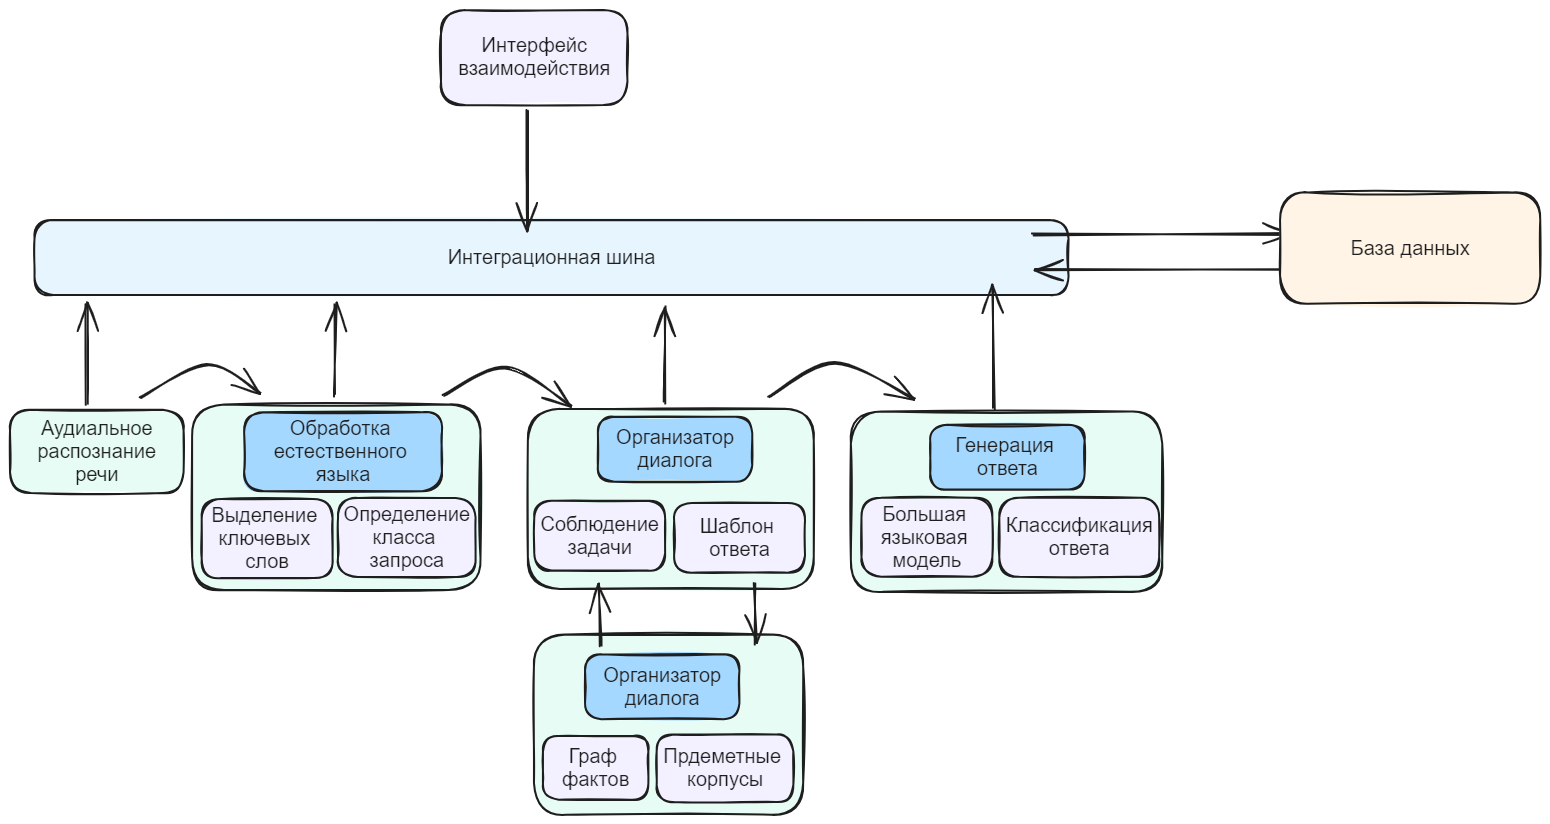
\includegraphics[width=0.85\textwidth]{assets/work/arch/modern_system.excalidraw.png}
    \caption{Модульная система позволяет эффективно организовывать командную работу.}
    \label{modular}
\end{figure}
В текущей практике шаблоны ответов заменяются на большие языковые модели. Такой подход позволяет повысить метрические показатели
удовлетворенности диалоговыми системами \cite{zhao2023survey}. Исследователи связывают преимущества с обилием знаний, полученных моделями при обучении.
Большие языковые модели эвристически понимают задачи пользователя, при необходимости умеют уточнять его потребности и 
могут быть адаптированы путем примеров без потребности в обучении \cite{wang2020generalizing}.

Разработанный в рамках работы ассистент включает в себя три основных компонента:
 \begin{itemize}
    \item модуль исключение ненормативной лексики и неэтичных изображений;
    \item большая языковая модель;
    \item модуль принятия решения о сложности задания для пользователя.
\end{itemize}

\begin{figure}[h]
    \centering
    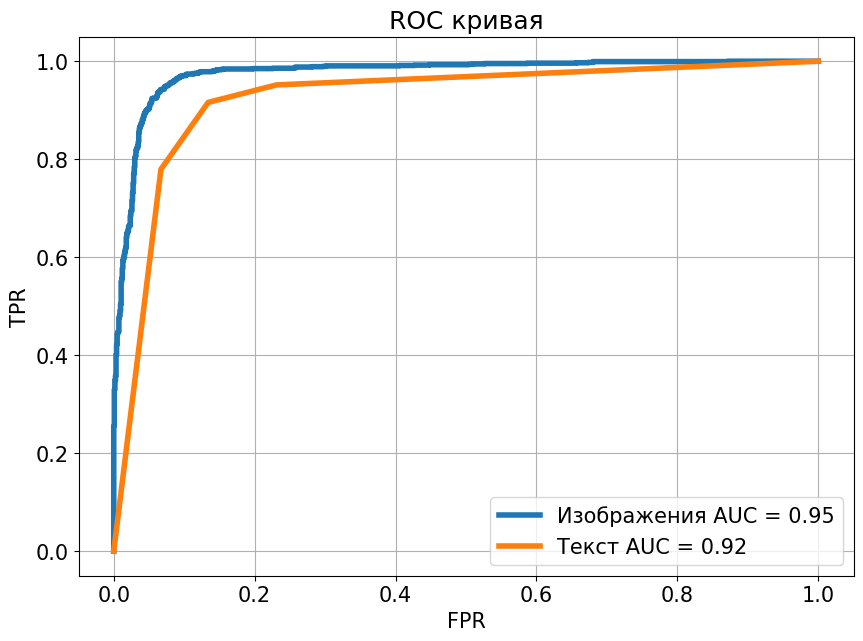
\includegraphics[width=0.7\textwidth]{assets/work/arch/detoxifier.png}
    \caption{Адаптация модуля CLIP позволила достичь высоких метрических результатов выделения неприемлемых изображений и фрагментов текста }
    \label{detox}
\end{figure}

Пресечение использования ненормативной лексики было выполнено с помощью морфологического анализатора текста  
PyMorphy \cite{Korobov2015morph}. Для исключения неэтичных по содержанию предложений и изображений был адаптирован 
бимодальный кодировщик CLIP \cite{radford2021learning}.
Преимущество работы кодировщиком заключается в определении негативного содержания в контексте \cite{bogoradnikova2021multilingual}. Использованные алгоритмы гарантируют исключение бранных слов 
и выделяют с высоким качеством неприемлемые по смыслу фрагменты текста и иллюстрации (табл. \ref{profanity_table}).

\begin{table}
    \centering
    \begin{tabular}{||c | c |c||} 
     \hline
     \text{Параметр} & \text{Текст} & \text{Изображения} \\
     \hline\hline
     \text{ROC AUC, \%} &  92.0 & 95.0 \\ 
     \hline
    \end{tabular}
    \caption{Метрические показатели }
    \label{profanity_table}
\end{table}

В качестве большой языковой модели была использована архитектура Llama3 \cite{llamatouvron2023}. 
Это наиболее продвинутая открытая модель, 
способная к общение на более чем ста языках мира. Ассистент вежлив в общении, внимателен к эмоциям собеседника и имеет обширные знания о мире.
В диалоговой системе ассистент следит за эмоциональным откликом обучающегося на материал,
узнает ее причину и в случае фиксации несоразмерной уровню нагрузки сообщает управляющей системе о потребности изменения сложности.
Также в задачи ассистента входят рекомендации по обучению и методической литературе для ознакомления.

Для поддержания оптимального уровня сложности используются байесова модели рейтинга, скалярно определяющая сложность
задания и уровень знаний учащегося. Принципиально система состоит из определения вероятности решения задачи с заданной сложностью
и правила обновления рейтинга согласно результату решения. Преимуществом таких систем является возможность обновления рейтинга 
учащегося в реальном времени.

Наиболее известной рейтинговой системой является модель Брэдли-Терри \cite{bradley1952rank}:
\begin{equation}
    p(i \succ j) = \frac{\theta_i}{\theta_i +\theta_j},
\end{equation}
где $\theta_i$ --- текущий уровень знаний учащегося, $\theta_j$ --- сложность задачи. Строгое правило пересчета требует
учета всех экспериментальных данных и может быть вычислительно затратным \cite{hunter2004mm}. Поэтому на практике 
используется перепараметризация модели $\theta = \exp(\frac{\nu}{\sigma})$, где $\sigma$ задает представления о 
волатильности данных:
\begin{equation}
    p(i \succ j) = \frac{1}{1 + \exp(\frac{\nu_i-\nu_j}{\sigma})}.
\end{equation}
Полученная модель соответствует модели Эло \cite{elo1967proposed} c правилом пересчета:
\begin{equation}
    \theta_i^{(t+1)} = \theta_i^{(t)} + \sigma,
\end{equation}
где $t$ задает номер пересчета. Таким образом, система стимулирует к решению более сложных задач, 
требующих освоения новых знаний.
Прогресс обучающегося согласно предложенной системы может быть статистически наблюдаем как 
повышение доли успеха в решении задач. 

